\subsection{Fiducial Volume}
\label{sec:Systematics_FiducialVolume}
A one-track per spill sample of beam MC has been used 
to extract the X and Y vertex resolution. 
Fig. \ref{fig:fiducialResolution} shows the X and Y coordinate resolution 
for Run 1 as determined by MC. 
The resolution is defined as the reconstructed position 
minus the true vertex position. The different X and Y resolution plots 
were fitted to a Breit-Wigner function which yielded in a FWHM 
that corresponds to a $\sigma$ of 5.7 mm and 7.2 mm respectively. \\

\begin{figure}[ht]
\centering
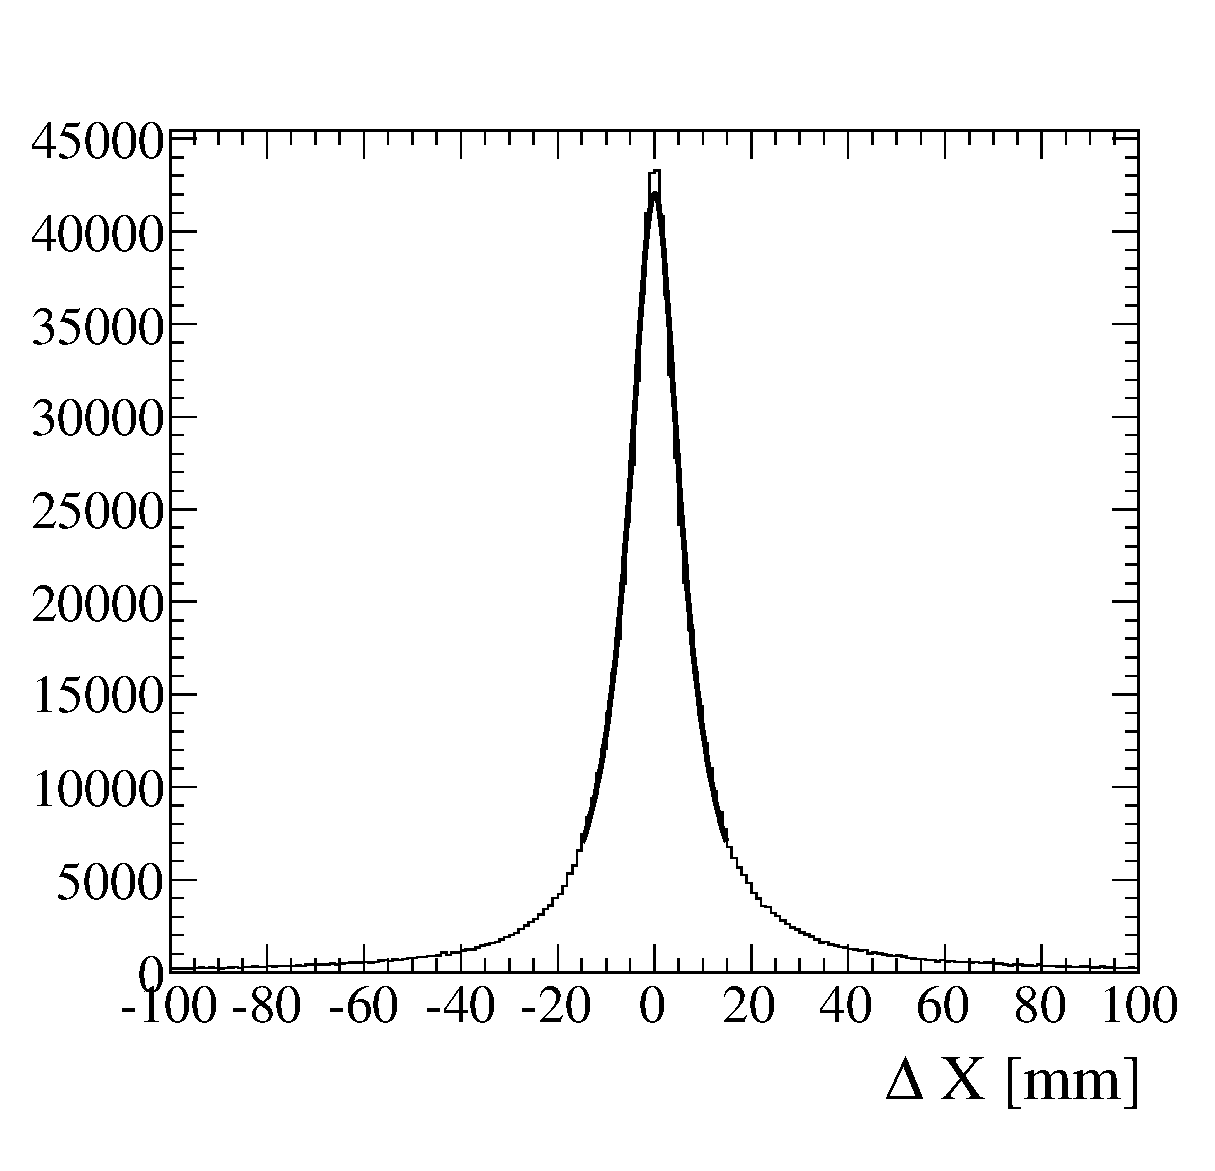
\includegraphics[width=2in]{Figures/P0DTrack-XResolution-Run4.eps}
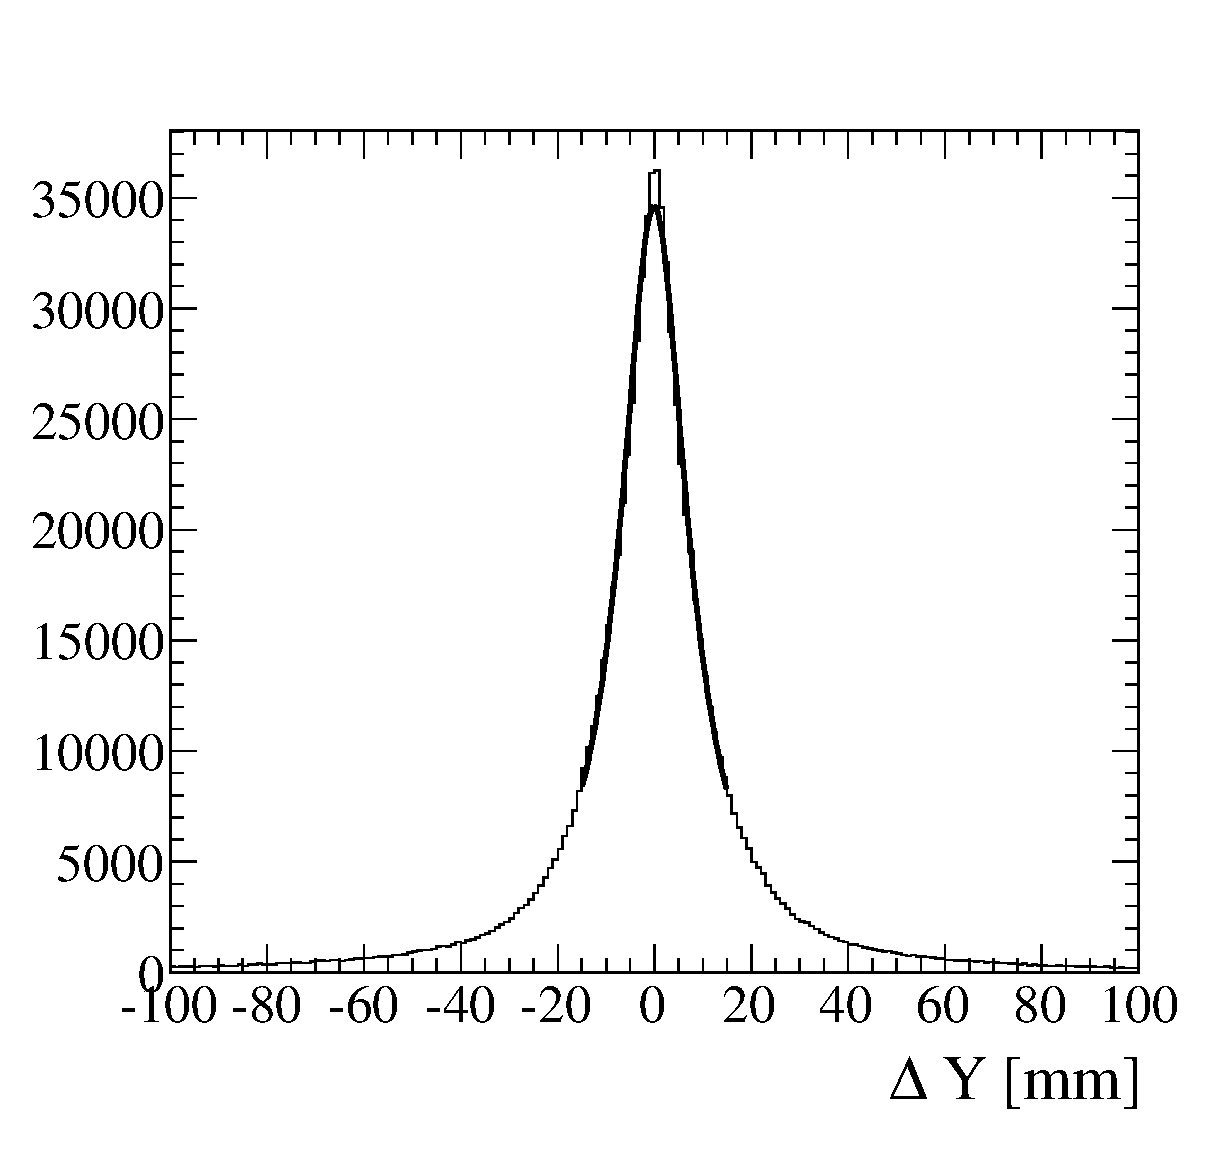
\includegraphics[width=2in]{Figures/P0DTrack-YResolution-Run4.eps}
\caption{Resolution of start position of Reconstructed - MC truth. 
On the Left (Right) is the X(Y) distribution.} 
\label{fig:fiducialResolution}
\end{figure}

To extract the FV systematic values we have simultaneously varied
all of our FV boundaries 
outside and inside, 
by $\pm$10 mm (which was a conservative $\pm\sigma$) 
in both X and Y coordinates and by 
%in the case of the Z coordinate we have varied the boundaries 
$\pm 1 $ layer in the Z coordinate.
The decision to vary the Z coordinate by one readout layer 
is due to the fact that 
each \p0dule has an X layer and a Y layer, 
%, which are named 
%in the reconstruction level as X node and Y node. 
%The 
where the WT FV excludes the most upstream X layer 
and the most downstream Y layer. \\
%Therefore we have chose to vary the Z coordinate by one readout layer.\\

We recalculated our Data-to-MC ratios for the outside and inside cases 
and extracted from these the corresponding systematic values. 
Tables \ref{tab:FVSystematicsWaterIn} and \ref{tab:FVSystematicsWaterOut} 
summarizes these values for 
the combination of both Water-in and Water-out  periods respectively. 
It was found that the inside variation yielded a value of $-$0.0057 
%for both runs 
while the outside variation gave a value of $+$0.0049.
% and +0.4\% 
%for run1 and run 2 respectively.

\begin{table}[h]
\centering
\begin{tabular}{ccc}\toprule
 & & Water-in \\
%\hline
\cline{3-3}
Outside & & $+$0.00867 \\
Inside & & $-$0.00160 \\
\bottomrule
\end{tabular} 
\caption{The fiducial volume systematics for the combined 
Run 1, Run 2 and Run4 Water-in periods. 
Outside (Inside) corresponds to the case were the boundaries were 
varied outside (inside) the official ones. }
\label{tab:FVSystematicsWaterIn}
\end{table}

\begin{table}[h]
\centering
\begin{tabular}{ccc}\toprule
 & & Water-out \\
%\hline
\cline{3-3}
Outside & & $+$0.00294 \\
Inside & & $+$0.00035 \\
\bottomrule
\end{tabular} 
\caption{The fiducial volume systematics for the combined 
Run 2, Run 3 and Run4 Water-out periods. 
Outside (Inside) corresponds to the case were the boundaries were 
varied outside (inside) the official ones. }
\label{tab:FVSyatematicsWaterOut} 
\end{table}

There are a few other possible effects we must consider. One is the effect of hit reconstruction efficiency when making a FV cut. This has been shown to be negligible in Section \ref{sec:Systematics_HitEfficiency}. Another is the possibility that the vertex resolution in Data is different from that in MC. However, we note that small differences in the width of the vertex resolution will not translate to a systematic uncertainty. As long as the vertex resolution (i.e. the residual distribution) is symmetric, the number of true out-of-FV events that get `smeared' into the FV will cancel out with the number of true in-FV event that get `smeared' out of the FV. This is the case regardless of any differences between the Data and MC vertex resolution distributions. Examining the matching parameter distributions (Figures \ref{fig:eff_dR} and \ref{fig:dRetcSM}) from Sections \ref{sec:CosmicsEfficiency} and \ref{sec:SMeff}, we can draw some conclusions on the vertex resolution in data. The backwards projected Tracker track provides a best guess for where the true position of the \p0d node should be, so the $\Delta Y$ and $\Delta X$ residuals mimic the vertex resolution. We see that the Data and MC residuals have similar widths (see Table \ref{tab:FitdY} for an example) and more importantly, are symmetric. This indicates that vertex resolution has negligible effect on the Fiducial Volume systematic.


